\documentclass[../../main.tex]{subfiles}
\begin{document}
\section{Introduction}
In this chapter, the Finite Element Method (FEM) is applied to the models of this dissertation, presented in Chapter 1. The goal of this chapter is to obtain an algorithm that can be used to calculate the eigenvalues and eigenvectors for the models. This is in preparation of chapter 6, where the eigenvalues and eigenvectors of the models are compared.

In chapter 4, a method was discussed to obtain the eigenvalues and eigenvectors for the Timoshenko beam model. Therefore it is not necessary to apply the Finite Element Method on the Timoshenko model to obtain the eigenvalues and eigenvectors. The Finite Element Method is applied to the two-dimensional and three-dimensional models.

The outline of the chapter is as follows.
\begin{itemize}
	\item[] Section \ref{sec:FEM:2D} FEM for a cantilever two-dimensional elastic body. This is problem 2D-1 in section \ref{ssec:2D_Model:ModelProblem}.
	\item[] Section \ref{sec:FEM:3D} FEM for a cantilever three-dimensional elastic body. This is problem 3D-1 in section \ref{ssec:3D_Model:ModelProblems}.
	\item[] Section \ref{sec:FEM:Plate} FEM for a cantilever Reissner-Mindlin plate. This is problem P-1 in section \ref{ssec:P_Model:ModelProblems}.
\end{itemize}

\section{A cantilever two-dimensional body} \label{sec:FEM:2D}
Consider a cantilever two-dimensional elastic body, with a rectangular cross-section.

\subsubsection{Reference configuration for rectangular cross-section}\label{sssec:2D_Model:RefConf}
Let $\{e_1,e_2\}$ be a right-handed orthonormal basis for $R^2$. Denote the elastic body by $\Omega \in R_2$, with $(0,0)$ as the point of reference. For a rectangular cross-section, the body $\Omega$ can be described as,
\begin{eqnarray*}
	\Omega = \left \{ x \in E_2 \ | \ 0 \leq x_1 \leq 1, \ -\frac{h}{2} \leq x_2 \leq \frac{h}{2} \right \},
\end{eqnarray*} where $\partial \Omega$ denotes the boundary of $\Omega$. The boundary $\partial \Omega$ can be divided into the four distinct lines (or edges) as follows:

\noindent\begin{minipage}{.5\linewidth}
	\begin{eqnarray*}
		\Sigma:& \quad x_1 &= 0\\
		\Gamma_3:& \quad x_1 &= 1
	\end{eqnarray*}
\end{minipage}%
\begin{minipage}{.5\linewidth}
	\begin{eqnarray*}
		\Gamma_1:& \quad x_2 &= -{h}/{2}\\
		\Gamma_2:& \quad x_2 &= {h}/{2}
	\end{eqnarray*}
\end{minipage}

In this configuration, the body is clamped rigidly to the surface at $x_1 = 0$ denoted as $\Sigma$ and the body is free-hanging on the other boundaries denoted by $\Gamma$.

\subsubsection{Cantilever elastic body}
Consider a two-dimensional elastic body clamped rigidly to a surface at $x_1 = 0$. The body is free-hanging on the other boundaries. This is Problem 2D-1 in section \ref{ssec:2D_Model:ModelProblem}.
\FloatBarrier
\begin{figure}[h!]
	\centering
	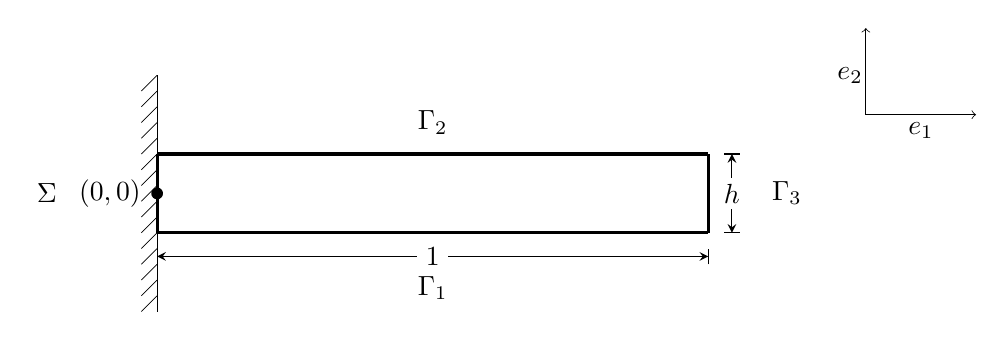
\begin{tikzpicture}
		
		\draw[line width = 0.4mm] (0,0.5) -- (7,0.5);
		\draw[line width = 0.4mm] (0,-0.5) -- (7,-0.5);
		\draw[line width = 0.4mm] (7,-0.5) -- (7,0.5);
		\draw[line width = 0.4mm] (0,-0.5) -- (0,0.5);
		
		\draw[line width = 0.1mm] (0,1.5) -- (0,-1.5);
		
		\draw[line width = 0.1mm] (0,1.5) -- (-0.2,1.3);
		\draw[line width = 0.1mm] (0,1.3) -- (-0.2,1.1);
		\draw[line width = 0.1mm] (0,1.1) -- (-0.2,0.9);
		\draw[line width = 0.1mm] (0,0.9) -- (-0.2,0.7);
		\draw[line width = 0.1mm] (0,0.7) -- (-0.2,0.5);
		\draw[line width = 0.1mm] (0,0.5) -- (-0.2,0.3);
		\draw[line width = 0.1mm] (0,0.3) -- (-0.2,0.1);
		\draw[line width = 0.1mm] (0,0.1) -- (-0.2,-0.1);
		\draw[line width = 0.1mm] (0,-0.1) -- (-0.2,-0.3);
		\draw[line width = 0.1mm] (0,-0.3) -- (-0.2,-0.5);
		\draw[line width = 0.1mm] (0,-0.5) -- (-0.2,-0.7);
		\draw[line width = 0.1mm] (0,-0.7) -- (-0.2,-0.9);
		\draw[line width = 0.1mm] (0,-0.9) -- (-0.2,-1.1);
		\draw[line width = 0.1mm] (0,-1.1) -- (-0.2,-1.3);
		\draw[line width = 0.1mm] (0,-1.3) -- (-0.2,-1.5);
		
		\node at (7.3,0) {$h$};
		\draw[-stealth] (7.3,0.2) -- (7.3,0.5);
		\draw (7.2,0.5) -- (7.4,0.5);
		\draw[-stealth] (7.3,-0.2) -- (7.3,-0.5);
		\draw (7.2,-0.5) -- (7.4,-0.5);
		
		\node at (3.5,-0.8) {$1$};
		\draw[stealth-] (0,-0.8) -- (3.3,-0.8);
		\draw[stealth-] (7,-0.8) -- (3.7,-0.8);
		\draw (7,-0.9) -- (7,-0.7);
		
		\draw[line width = 0.1mm,->] (9,1) -- (10.4,1);
		\draw[line width = 0.1mm,->] (9,1) -- (9,2.1);
		\node at (9.7,0.8) {$e_1$};
		\node at (8.8,1.5) {$e_2$};
		
		\node at (-0.6,0) {$(0,0)$};
		\node at (0,0)[circle,fill,inner sep=1.5pt]{};

		% Add Σ at x_1 = 0
		\node at (-1.4,0) {$\Sigma$};
		
		% Add Γ₁ at x_2 = -h/2
		\node at (3.5,-1.2) {$\Gamma_1$};
		
		% Add Γ₂ at x_2 = h/2
		\node at (3.5,0.9) {$\Gamma_2$};
		
		% Add Γ₃ at x_1 = 1
		\node at (8,0) {$\Gamma_3$};
		
	\end{tikzpicture}
	\caption{A cantilever two-dimensional elastic body.}
\end{figure} 
\FloatBarrier

In section \ref{ssec:2D_Model:VariationalForm} the variational problem for the two dimensional cantilever model is derived and refered to as Problem 2D-1V. Some of the results from section \ref{sec:2D_Model} are repeated here for convenience. Using the reference configuration, these results are rewritten from a general form to a model specific form.

\subsubsection{Problem 2D-1V}\label{sssec:2D_Model:Problem2D1VChp5}
Find a function $u$ such that for all $t>0$, $u \in T(\Omega)$ and 
\begin{align}
	c(u,\phi) = -b(u,\phi) + (Q,\phi) \label{eq:2D_Model:Problem2D1VEqChp5}
\end{align}
for all $\phi \in T(\Omega)$. With the test function space 
\begin{eqnarray*}
	T(\Omega) & = & \left\{ \phi \in C^1(\bar{\Omega}) \ | \ \phi = 0 \ \textrm{ on } \ \Gamma \right\}.
\end{eqnarray*}

The bilinear forms and integral function is defined by
\begin{eqnarray}
	b(u,\phi) & = & \int_\Omega~c_1\textrm{Tr}({\cal E}\Phi)+ c_2\textrm{Tr}({\cal E})
	\textrm{Tr}(\Phi) ~dA, \label{eq:2D_Model:BilinearChp5}\\
	c(\partial_t^2 u,\phi) & = & \int_\Omega~ (\partial^2_t u) \cdot \phi~dA, \label{eq:2D_Model:Bilinear_cChp5}\\
	(f,g) &=& \int_{\Omega} f\cdot g \ dA, \label{eq:2D_Model:Bilinear_intChp5}
\end{eqnarray}
with $\displaystyle c_1 = \frac{1}{\gamma(1+\nu)}$ and $\displaystyle c_2 = \frac{\nu}{\gamma(1-\nu^2)}$.

Using the reference configuration, the constitutive equations and the bilinear form $b$ can be rewritten into a model specific form.

\subsubsection{Constitutive equations:}
\begin{eqnarray}
	\sigma_{11} & = & \frac{1}{\gamma(1-\nu^2)}(\partial_1 u_1 + \nu \partial_2 u_2) \label{CE1} \\
	\sigma_{22} & = & \frac{1}{\gamma(1-\nu^2)}(\partial_2 u_2 + \nu \partial_1 u_1) \label{CE2} \\
	\sigma_{12} & = & \frac{1}{2\gamma(1+\nu)}(\partial_1 u_2 + \partial_2 u_1) \label{CE3}
\end{eqnarray}

\subsubsection{Bilinear form:}
\begin{align}
	b(u,\phi) & = & \frac{1}{\gamma(1-\nu^2)}\int_{\Omega} (\partial_1 u_1 \partial_1 \phi_1 + \partial_2 u_2 \partial _2 \phi_2 + \nu\partial_1 u_1 \partial_2\phi_2 + \nu \partial_2 u_2 \partial_1 \phi_1 ) \ dA \nonumber\\
	& + & \frac{1}{2\gamma(1+\nu)}\int_{\Omega} (\partial_1 u_2 \partial_1 \phi_2 + \partial_1 u_2 \partial_2 \phi_1 + \partial_2 u_1 \partial_1\phi_2 + \partial_2 u_1 \partial_2\phi_1) \ dA.
\end{align}

\subsection{Weak variational form}
Define the inertia space $V$ as the closure of $T(\Omega)$ in $H := H^1(0,1)\times H^1(0,1)$. Denote $X = L^2(0,1)\times L^2(0,1)$. The inertia space is $W  = X$ with norm $||\cdot||_W = \sqrt{c(\cdot,\cdot)}$.

\subsubsection{Problem 2D-1WV}
Find a function $u$ such that $\forall \ t > 0$, $u \in V$ with $\partial_t^2 u \in W$ and
\begin{eqnarray*}
	c(u,v) + b(u,v) & = & (Q,v)
\end{eqnarray*}
for all $v\in V$.

See Chapter 2 for the existence theory.

\subsection{Galerkin approximation}\label{2d_FEM_G}
To be able to apply the Finite Element Method to Problem 2D-1V, the body $\Omega$ needs to be discretised. This is done by dividing the body $\Omega$ into discrete shapes, called elements. There are various types of shapes of elements that can be used. Since the body $\omega$ is has a rectangular cross-section, rectangular elements are the simplest elements to use.

Divide the reference configuration $\Omega$ into a grid of rectangular elements, such that there are $n = n_1\times n_2$ nodes.

Define a set of $n$-dimensional linear independent basis functions. For the two dimensional model, the basis functions can be defined by the set $$B = \left\{\langle\phi_1, 0\rangle, \langle\phi_2, 0\rangle,...,\langle\phi_{n}, 0 \rangle,\langle 0,\phi_1\rangle,\langle 0 ,\phi_2\rangle,...,\langle 0,\phi_{n}\rangle \right\}.$$ 

These functions are chosen as bi-cubic functions $\phi_i$. Simpler bi-linear functions can also be used, however the use of the bi-cubic basis functions results in faster convergence and also the benefit of obtaining the derivatives of the solution at the expense of more complexity.

The subset of basis functions $B$ that satisfies all the conditions of the test function space $T(\Omega)$ are called the admissible basis functions. Denote the admissible basis functions by $\delta_j$, where each $\delta_j$ is a unique element of $B$. The admissible basis functions can be numbered and expressed as the set $A = \left \{\delta_1, \delta_2,..., \delta_k \right\}$ for some $k \leq 2n$.\\ 

Define the space
\begin{eqnarray*}
S^h & = & \textrm{span}\left(\left\{\delta_i \ | \ i = 1,2,...,k \right\} \right).
\end{eqnarray*}

For each function $u^h \in S^h$, $u^h$ can be expressed as
\begin{eqnarray*}
	u^h = \sum_{i = 1}^{k} u_i(t) \delta_{i}(x).
\end{eqnarray*}

Substitution of $u^h$ into Problem 2D-1V, results in the following Galerkin Approximation, denoted by Problem 2D-1G.

\subsubsection{Problem 2D-1G}
Find a function $u^h$ such that for all $t>0$, $u^h \in S^h$ and
\begin{eqnarray*}
	(u^h, \phi_i) & = & -b(u^h,\phi_i) + (Q^I, \phi_i)
\end{eqnarray*} for $i = 1,2,...,k$. $Q^I$ is scalar vector obtained after interpolating the function $Q$ over the rectangular grid $\Omega$. i.e. $Q^I_{i,j} = Q(x_i,x_j)$ for $i = 1,2,...,n_1$ and $j = 1,2,...,n_2$.

\subsection{System of differential equations}\label{ssec:2DFEM:DE}

Consider the following standard Finite Element Method matrices
\subsubsection{FEM matrices}
\noindent\begin{minipage}{.5\linewidth}
	\begin{eqnarray*}
		\mathbf{M}_{j,i} & = & \int_{\Omega} \phi_i \phi_j ~dA \\
		\mathbf{{K}_{11}}_{j,i} & = & \int_{\Omega} \partial_1\phi_i \partial_1\phi_j~dA\\
		\mathbf{{K}_{22}}_{j,i} & = & \int_{\Omega} \partial_2\phi_i \partial_2\phi_j~dA
	\end{eqnarray*}
\end{minipage}%
\begin{minipage}{.5\linewidth}
	\begin{eqnarray*}
		\mathbf{{K}_{12}}_{j,i} & = & \int_{\Omega} \partial_2\phi_i \partial_1\phi_j~dA\\
		\mathbf{{K}_{21}}_{j,i} & = & \int_{\Omega} \partial_1\phi_i \partial_2\phi_j~dA
	\end{eqnarray*}
\end{minipage}
for $i,j = 1,2,...,k$.

And 
\begin{eqnarray*}
	{M_{F}}_{j,i} = \int_{\Omega}  \phi_i \phi_j~dA
\end{eqnarray*}

for $i = 1,2,...,k$ and for $j =1,2,...,2n$.

Define the following matrices:
\begin{eqnarray*}
	K_1 & = & \frac{1}{\gamma(1-\nu^2)} \mathbf{K_{11}} + \frac{1}{2\gamma(1+\nu)}\mathbf{K_{22}} \label{eq:2DFEM:K1} \\
	K_2 & = & \frac{\nu}{\gamma(1-\nu^2)} \mathbf{K_{21}} + \frac{1}{2\gamma(1+\nu)}\mathbf{K_{12}}\label{eq:2DFEM:K2}\\
	K_3 & = & \frac{\nu}{\gamma(1-\nu^2)} \mathbf{K_{12}} + \frac{1}{2\gamma(1+\nu)}\mathbf{K_{21}}\label{eq:2DFEM:K3}\\
	K_4 & = & \frac{1}{\gamma(1-\nu^2)} \mathbf{K_{22}} + \frac{1}{2\gamma(1+\nu)}\mathbf{K_{11}}\label{eq:2DFEM:K4}
\end{eqnarray*}

Using the standard FEM matrices and matrices $K_1$-$K_4$, the following concatenated matrices are defined.
\begin{eqnarray}
	\begin{aligned}
		K = 
		\begin{bmatrix}
			K1 & K2\\
			K3 & K4
		\end{bmatrix}
	\end{aligned}
	\ \ \ \ \ \ \ \ \
	\begin{aligned}
		M_f = 
		\begin{bmatrix}
			M_{F} & O_{F}\\
			O_{F} & M_{F}
		\end{bmatrix}
	\end{aligned}\label{eq:2DFEM:K+M}
\end{eqnarray}

\begin{eqnarray}
	M = 
	\begin{bmatrix}
		\mathbf{M} & O \\
		O & \mathbf{M}
	\end{bmatrix}\label{eq:2DFEM:M}
\end{eqnarray}

The matrices ${O}$ and ${O_f}$ are the zero matrices of the same size as $\mathbf{M}$ and ${M_f}$ respectively.

Using \eqref{eq:2DFEM:K+M} and \eqref{eq:2DFEM:M}, Problem 2D-1G is rewritten as a system of ordinary differential equations. This system is referred to as Problem 2D-1ODE.

\subsubsection{Problem 2D-1ODE}
Find a function $\bar{u} \in S^h$ such that
\begin{eqnarray}
	M\ddot{\bar{u}} & = & K\bar{u} + M_{f}Q^I.
\end{eqnarray} With $\bar{u}$ in the form $\bar{u} = \langle u, \partial_1 u, \partial_2 u, \partial_{12} u \rangle$.

\textbf{Remark} This form of $\bar{u}$ is determined by the use of the bi-cubic basis functions.

\subsection{Eigenvalue problem}\label{2dFEM_EP}
For the eigenvalue problem, assume that there is no external force, $M_{f}Q^I = 0$, so that 
\begin{eqnarray}
		M\ddot{\bar{u}} & = & K\bar{u}.\label{eq:2DFEM:M2}
\end{eqnarray}
It is known that a system of ordinary differential equations has a general solution of the form $e^{rt}$. Suppose that $\bar{w} = e^{\lambda t} \bar{u}$ is a solution for \eqref{eq:2DFEM:M2}. In this solution, $\lambda$ is an eigenvalue and $\bar{u}$ a corresponding eigenfunction. Substitution into \eqref{eq:2DFEM:M2} results in
\begin{eqnarray*}
	M\lambda e^{\lambda t}\bar{u} & = & Ke^{\lambda t}\bar{u}.
\end{eqnarray*}
Since $e^{\lambda t} > 0$ for all values of $\lambda t$, we can cancel it from both sides of the equation and formulate the eigenvalue problem Problem 2D-1E.

\subsubsection{Problem 2D-1E}
Find a real number $\lambda$ and a function $\bar{u} \in S^h$ such that
\begin{eqnarray}
	M\lambda{\bar{u}} & = & K\bar{u}.
\end{eqnarray}

\end{document}


Divide the reference configuration $\Omega$ into $n_1\times n_2$ nodes in a rectangular grid.\\

Consider a set of 
For this dissertation, we consider bi-cubic basis functions, however bi-linear basis functions can also be used.

Consider a $n$-dimensional set of linearly independent two-dimensional scalar valued functions, denoted $\delta_i$. In this dissertation, these functions are chosen as bi-cubic functions, however simpler bi-linear functions can also be used.\\

The functions in the set that satisfies the conditions of the test function space $T(\Omega)$ are called the admissible basis functions. Number these admissible basis functions $\delta_1, \delta_2,...,\delta_k$ for some $k \leq n$.

Let $S^h$ be a $2k$-dimensional subset of $T(\Omega)$ such that
\begin{eqnarray*}
	S^h & = & \textrm{span}\left \{[\delta_1 \ 0], [\delta_2 \ 0],...,[\delta_k \ 0],[0 \ \delta_1],[0 \ \delta_2],...,[0 \ \delta_k] \right\}.
\end{eqnarray*}



Let $S^h$ be a $2k$-dimensional subset of $T(\Omega)$ such that
\begin{eqnarray*}
	S^h & = & \textrm{span}\left \{[\delta_1 \ 0], [\delta_2 \ 0],...,[\delta_k \ 0],[0 \ \delta_1],[0 \ \delta_2],...,[0 \ \delta_k] \right\}.
\end{eqnarray*}


he body $\Omega$ is divided into an $n_1\times n_2$ rectangular grid. Let $x_i^* = \langle x_1, x_2 \rangle \in \Omega$ where $\delta_{i}(x_1,x_2) = 1$. Define $\bar{x} = \langle x_1^*, x_2^*,...,x_k^* \rangle$. For each solution $u$ of Problem 2D-1V let $u^h$ denote the projection of $u$ into the finite dimensional space $S^h$. Each function $u^h=\langle u_1^h,u_2^h\rangle$ in S$^h$ can be expressed as
\begin{eqnarray*}
	u_1^h(\bar{x},t) = \sum_{i = 1}^{k} u_{1}(x_i^*,t) \delta_{i}(\bar{x}) \ \ \textrm{ and } \ u_2^h(\bar{x},t) = \sum_{i = 1}^{k} u_{2}(x_i^*,t) \delta_{i}(\bar{x}).
\end{eqnarray*}
